%
% File acl2017.tex
%
%% Based on the style files for ACL-2015, with some improvements
%%  taken from the NAACL-2016 style
%% Based on the style files for ACL-2014, which were, in turn,
%% based on ACL-2013, ACL-2012, ACL-2011, ACL-2010, ACL-IJCNLP-2009,
%% EACL-2009, IJCNLP-2008...
%% Based on the style files for EACL 2006 by 
%%e.agirre@ehu.es or Sergi.Balari@uab.es
%% and that of ACL 08 by Joakim Nivre and Noah Smith

\documentclass[11pt,a4paper]{article}
\usepackage[hyperref]{acl2017}
\usepackage{times}
\usepackage{latexsym}
\usepackage{url}


%% not part of the template

\usepackage{graphicx}
\usepackage{bm}
\usepackage{multirow}
\usepackage{pifont}
\usepackage{amsmath} 
\usepackage{amsthm}
\usepackage{algorithm}
\usepackage{algpseudocode}
\usepackage{varwidth}
\newcommand{\cmark}{\ding{51}}
\newcommand{\xmark}{\ding{55}}
\newtheorem{theorem}{Theorem}
\newtheorem{example}{Example}
\algnewcommand{\LeftComment}[1]{\Statex \(\triangleright\) #1}

% make itemset denser
\usepackage{enumitem}
\setlist[itemize]{itemsep=1pt, topsep=1pt}

\setlength{\abovedisplayskip}{0pt}
\setlength{\belowdisplayskip}{0pt}
\setlength{\abovedisplayshortskip}{0pt}
\setlength{\abovedisplayshortskip}{0pt}

\setlength{\textfloatsep}{5pt plus .5pt minus 1pt}
\setlength{\floatsep}{5pt plus .5pt minus 1pt}
\setlength{\intextsep}{5pt plus .5pt minus 1pt}

%\aclfinalcopy % Uncomment this line for the final submission
%\def\aclpaperid{***} %  Enter the acl Paper ID here

%\setlength\titlebox{5cm}
% You can expand the titlebox if you need extra space
% to show all the authors. Please do not make the titlebox
% smaller than 5cm (the original size); we will check this
% in the camera-ready version and ask you to change it back.

\newcommand\BibTeX{B{\sc ib}\TeX}


\title{A FOFE-based Local Detection Approach for Named Entity Recognition and Mention Detection}

\author{Mingbin Xu \and Hui Jiang \\
	Department of Electrical Engineering and Computer Science \\
	Lassonde School of Engineering, York University \\
	4700 Keele Street, Toronto, Ontario, Canada\\
	{\tt xmb@cse.yorku.ca} \and  {\tt hj@cse.yorku.ca}
	%\\\And
	%Hui Jiang \\
	%Lassonde School of Engineering, \\
	%York University \\
	%{\tt hj@eecs.yorku.ca} \\
}

\date{}

\begin{document}
\maketitle


\begin{abstract}
	In this paper, we study a novel approach for named entity recognition (NER) and mention detection (MD) in natural language processing. Instead of treating NER as a sequence labeling problem, we propose a new local detection approach, which relies on the recent fixed-size ordinally forgetting encoding (FOFE) method to fully encode each sentence fragment and its left/right contexts into a fixed-size representation. Subsequently, a simple feedforward neural network (FFNN) either rejects or predicts entity label for each individual fragment. The proposed method has been evaluated in several popular NER and MD tasks, including CoNLL 2003 NER task and  TAC-KBP2015 and TAC-KBP2016 Tri-lingual Entity Discovery and Linking (EDL) tasks. Our method has yielded pretty strong performance in all of these examined tasks. This local detection approach has shown many advantages over the traditional sequence labeling  methods.
\end{abstract}


\section{Introduction}

Natural language processing (NLP) plays an important role in artificial intelligence, which has been extensively studied for many decades. Conventional NLP techniques include the rule-based symbolic approaches widely used about two decades ago, and the more recent statistical approaches relying on feature engineering and statistical models. In the recent years, deep learning approach has achieved huge successes in many applications, ranging from speech recognition to image classification. It is drawing increasing attention in the NLP community. 

In this paper, we are interested in a fundamental problem in NLP, namely named entity recognition (NER) and mention detection (MD). NER and MD is a very challenging task in NLP, laying the foundation of almost every NLP application.
NER and MD is a task of identifying entities (named and/or nominal) from raw text, and classifying the detected entities into one of the pre-defined categories such as person (PER), organization (ORG), location (LOC), etc. Some tasks focus on named entities only, 
%for example, 
%\begin{quote}
%	\label{emp:4types}
%	\small
%	${[S.E.C.]}_{ORG}$ chief ${[Mary\ Shapiro]}_{PER}$ left ${[Washington]}_{LOC}$ in December .
%\end{quote}
while the others also detect nominal mentions. %, for example
%which are important for other NLP tasks such as co-reference resolution
%\begin{quote}
%	\label{emp:10types}
%	\small
%	$[Mark]_{PER}$ and his closest $[friend]_{PER\_N}$ $[Scarlet]_{PER}$, a cello $[player]_{PER\_N}$, joined the same music $[company]_{ORG\_N}$.
%\end{quote}
Moreover, nested mentions may need to be extracted too. For example, 
%\begin{quote}
%	\label{emp:nested-ex}
%	\small
%	He used to study in \\  ${[University\ of\ {[Toronto]}_{LOC}]}_{ORG}$.
%\end{quote}
\begin{quote}
	\small
	$[Sue]_{PER}$ and her $[brother]_{PER\_N}$ studied in ${[University\ of\ {[Toronto]}_{LOC}]}_{ORG}$. 
\end{quote}
where {\it Toronto} is a LOC entity, embedded in another longer ORG entity {\it University of Toronto}.

Similar to many other NLP problems, NER and MD is formulated as a sequence labeling problem, where a tag is sequentially assigned to each word in the input sentence. It has been extensively studied in the NLP community \cite{borthwick1998exploiting}. The core problem is to model the conditional probability of an output sequence given an arbitrary input sequence. Many hand-crafted features are combined with statistical models, such as conditional random fields (CRFs) \cite{nguyen2010kernel}, to compute conditional probabilities. More recently, some popular neural networks, including convolutional neural networks (CNNs) and recurrent neural networks (RNNs), are proposed to solve sequence labelling problems.
%under the popular sequence to sequence modeling framework. The relevant work will be briefly reviewed in Section \ref{sec_related_work}. 
In the inference stage, the learned models compute the conditional probabilities and the output sequence is generated by the 
%well-known 
Viterbi decoding algorithm \cite{Viterbi1967err}. 

In this paper, we propose a novel local detection approach for solving NER and MD problems. The idea can be easily extended to many other sequence labeling problems, such as chunking, part-of-speech tagging (POS). Instead of globally modeling the whole sequence in training and jointly decode the entire output sequence in test, 
our method examines all word segments (up to a certain length) in a sentence. A word segment will be examined individually based on the underlying segment itself and its left and right contexts in the sentence so as to determine whether this word segment is a valid named entity and the corresponding label if it is. 
This approach conforms to the way human resolves an NER problem. Given any word fragment and its contexts in a sentence or paragraph, people accurately determine whether this word segment is a named entity or not. People rarely conduct a global decoding over the entire sentence to make such a decision. 
The key to making an accurate local decision for each individual fragment is to have full access to the fragment itself as well as its complete contextual information. 
The main pitfall to implement this idea is that we can not easily encode the segment and its contexts in models since they are of varying lengths in natural languages. Many feature engineering techniques have been proposed but all of these methods will inevitably lead to information loss. 
In this work, we propose to use a recent fixed-size encoding method, namely fixed-size ordinally forgetting encoding (FOFE) \cite{zhang2015fixed}, to solve this problem.  The FOFE method is a simple recursive encoding method. FOFE theoretically guarantees (almost) unique and lossless encodding of any variable-length sequence. The left and the right contexts for each word segment are encoded by FOFE method, and then a simple neural network can be trained to make a precise recognition for each individual word segment based on the fixed-size presentation of the contextual information. This FOFE-based local detection approach is more appealing to NER and MD. Firstly, feature engineering is almost eliminated. 
%FOFE only relies on a single forgetting factor to encode any sequence. 
Secondly, under this local detection framework, nested mention is handled with little modification. Next, it makes better use of partially-labeled data available from many application scenarios. Sequence labeling model requires all entities in a sentence to be labeled. If only some (not all) entities are labeled, it is not effective to learn a sequence labeling model. However, every single labeled entity, along with its contexts, may be used to learn the proposed model. At last, due to the simplicity of FOFE, simple neural networks, such as multilayer perceptrons, are sufficient for recognition. These models are much faster to train and easier to tune. In the test stage, all possible word segments from a sentence may be packed into a mini-batch, jointly recognized in parallel on GPUs. This leads to a very fast decoding process as well.

In this paper, we have applied this FOFE-based local detection approach to several popular NER and MD tasks, including the CoNLL 2003 NER task and 
TAC-KBP2015 and TAC-KBP2016 Tri-lingual Entity Discovery and Linking (EDL) tasks.
Our proposed method has yielded strong performance in all of these examined tasks. 

\section{Related Work}
\label{sec_related_work}

It has been a long history of research involving neural networks (NN). In this section, we briefly review some recent NN-related research work in NLP, which may be relevant to our work. 

The success of word embedding \cite{mikolov2013distributed} encourages researchers to focus on machine-learned representation instead of heavy feature engineering in NLP. Using word embedding as the typical feature representation for words, NNs become competitive to traditional approaches in NER. 
%Many NLP tasks, such as NER, chunking and part-of-speech (POS) tagging can be formulated as sequence labeling tasks.
In \cite{collobert2011natural}, 
deep convolutional neural networks (CNN) and conditional random fields (CRF) are used to infer NER labels at a sentence level, where they still use many hand-crafted features to improve performance, such as capitalization features explicitly defined based on first-letter capital, non-initial capital and so on.

Recently, recurrent neural networks (RNNs) have demonstrated the ability in modeling sequences \cite{graves2012neural}. 
\newcite{huang2015bidirectional} built on the previous CNN-CRF approach by replacing CNNs with bidirectional Long Short-Term Memory (B-LSTM). 
Though they have reported improved performance, they employ heavy feature engineering in that work, most of which is language-specific. There is a similar attempt in \cite{rondeau2016lstm} with full-rank CRF. 
CNNs are used to extract character-level features automatically in \cite{dos2015boosting}. 

Gazetteer is a list of names grouped by the pre-defined categories.
%an NER system is targeting at. 
Gazetteer is shown to be one of the most effective external knowledge sources to improve NER performance \cite{tjong2003introduction}. Thus, gazetteer is widely used in many NER systems.  
In \cite{chiu2016named}, state-of-the-art performance on a popular NER task, i.e., CoNLL2003,  is achieved by incorporating  a large gazetteer. 
Different from previous ways to use a set of bits to indicate whether a word is in gazetteer or not, 
they have encoded a match in BIOES (Begin, Inside, Outside, End, Single) annotation, 
which captures positional information. 
%Their models also make advantage of word embeddings, character-level CNNs and CRFs. 

Interestingly enough, none of these recent successes in NER was achieved by a vanilla RNN. Rather, 
these successes are often established by sophisticated models combining CNNs, LSTMs and CRFs in certain ways. 
%In this paper, based on recent work in \cite{zhang2015fixed} and \cite{zhang2016compact},
%we propose a novel but simple solution to NER by applying DNN on top of FOFE-based features.
%This simpler approach can achieve performance very close to state-of-the-art on various NER and MD tasks, without using any external knowledge or feature engineering.

\begin{figure*}[t]
	\centering
	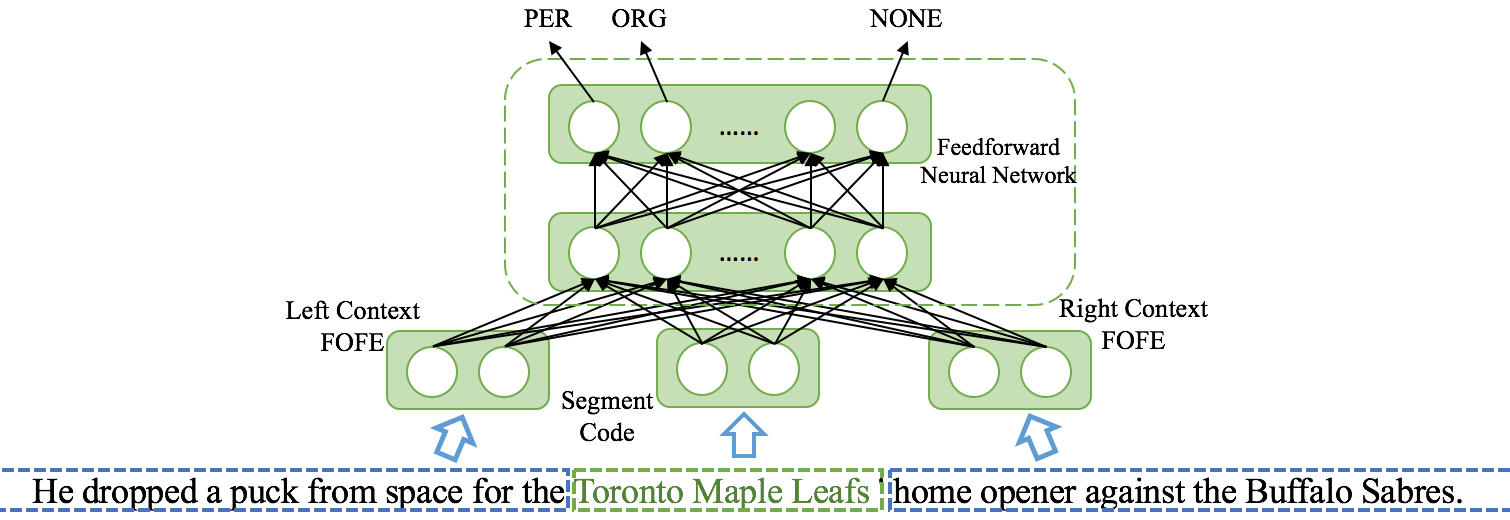
\includegraphics[width=0.86\linewidth]{figure-diagram-v5}
	\caption{Illustration of the local detection approach for NER using FOFE codes as input and an FFNN as model. The window currently examines the fragment of {\it Toronto Maple Leafs}. The window will scan and scrutinize all fragments up to $K$ words. }
	\label{Fig:FOFE-NER-diagram}
\end{figure*}


\section{Preliminary}

In this section, we will briefly review some background techniques, which are important to our proposed NER and mention detection approach. 

\subsection{Deep Feedforward Neural Networks}

It is well known that  neural network is a universal approximator under certain conditions \cite{hornik1991approximation}.
A feedforward neural network (FFNN) is a weighted graph with a layered architecture.
Each layer is composed of several nodes.
Successive layers are fully connected. Each node applies a function on the weighted sum of the lower layer.
%Formally, let $x_{n,j}$ denote the value of the $j$-th node in the
%$n$-th layer and $W^n_{i,j}$ denote the weight of the connection from
%$x_{n,i}$ to $x_{n+1,j}$. Then
%\begin{equation}
%z_{n+1,j} = \sum_i W^n_{i,j} x_{n,i}
%\end{equation}
%\begin{equation}
%x_{n+1,j} = \sigma\left(z_{n+1,j}\right)
%\end{equation}
%where $\sigma$ is the activation function, usually chosen to be 
%sigmoid:
%\begin{equation}
%\sigma(x) = \frac{1}{1 + e^{-x}}
%\end{equation}
%or 
%rectified linear unit (ReLU):
%\begin{equation}
%\sigma(x) = \max(0, x).
%\end{equation}
%For classification tasks, the outputs are normalized into a probability distribution by the so-called {\it soft-max} function, where the $i$-th node is computed as follows:
%\begin{equation}
%\sigma(x_i) =  \frac{\exp(x_i)}{\sum_{j} \exp(x_j)}.
%\end{equation}
An NN can learn by adjusting its weights in a process called back-propagation. 
%Suppose that we have already calculated the outputs given by an NN for any input.
%Let $E(y,t)$ be an error metric that measures how incorrect the output
%$y$ is with respect to the expected target output $t$. For each weight
%in NN, we may calculate:
%\begin{equation}
%\frac{\partial E}{\partial W^n_{i,j}} = \frac{\partial E}{\partial
%	\sigma} \frac{\partial \sigma}{\partial z_{i+1,j}} \frac{\partial
%	z_{i+1,j}}{\partial W^n_{i,j}}.
%\end{equation}
%Each weight may be adjusted to slowly reduce this error for each training
%example, and hence the NN learns to fit the input and the output. 
%This is accomplished by the following the update rule, where $\alpha$ is called the learning rate:
%\begin{equation}
%W^n_{i,j} := W^n_{i,j} - \alpha \frac{\partial E}{\partial
%	W^n_{i,j}}.
%\end{equation}
The learned NN may be used to generalize and extrapolate to new inputs that have not been seen during training.

\subsection{Fixed-size Ordinally Forgetting Encoding}

FFNN is a powerful computation model. 
However, it requires fixed-size inputs and 
lacks the ability of capturing long-term dependency. 
Because most NLP problems involves variable-length sequences of words, 
RNNs/LSTMs are more popular than FFNNs in dealing with these problems. 
The Fixed-size Ordinally Forgetting Encoding (FOFE), 
originally proposed in \cite{zhang2015fixed}, nicely overcomes the limitations of FFNNs because it 
can uniquely and losslessly encode a variable-length sequence of words into a fixed-size representation. 

Give a vocabulary $V$, each word can be represented by a one-hot vector. 
FOFE mimics bag-of-words (BOW) but incorporates a forgetting factor to capture positional information.
It encodes any sequence of variable length composed by words in $V$. 
Let $S = {w_1, w_2, w_3, ... , w_T}$ denote a sequence of $T$ words from $V$, 
and $\bm{e_t}$ be the one-hot vector of the $t$-th word in $S$, where $1 \leq t \leq T$.
The FOFE of each partial sequence $\bm{z_t}$ from the first word to the $t$-th word is recursively defined as:
\begin{equation}
\bm{z_t}=
\begin{cases}
\bm{0}, & \text{if}\ t = 0 \\
\alpha \cdot \bm{z_{t - 1}} + \bm{e_t}, & \text{otherwise}
\end{cases}  \label{eq_FOFE_formula}
\end{equation}
where the constant $\alpha$ is called forgetting factor, and it is picked between $0$ and $1$ exclusively. 
Obviously, the size of $\bm{z_t}$ is $|V|$, and it is irrelevant to the length of original sequence, $T$.

Here's an example. Assume that we have three words in our vocabulary, e.g. A, B, C, 
whose one-hot representations are $[1, 0, 0]$, $[0, 1, 0]$ and $[0, 0, 1]$ respectively. 
When calculating from left to right, the FOFE for the sequence 
"ABC" is $[{\alpha}^2, {\alpha}, 1]$, 
and that of 
"ABCBC" is $[{\alpha}^4, {\alpha} + {\alpha}^3, 1 + {\alpha}^2]$.

The word sequences can be unequivocally recovered from their FOFE representations \cite{zhang2015fixed}.
The uniqueness of FOFE representation is theoretically guaranteed
by the following two theorems: 
\begin{theorem}
	If the forgetting factor $\alpha$ satisfies $0 < \alpha \leq 0.5$, FOFE is unique for any countable vocabulary $V$ and any finite value $T$.
\end{theorem}
\begin{theorem}
	For $0.5 < \alpha < 1 $, given any finite value $T$ and any countable vocabulary $V$,
	FOFE is almost unique everywhere, except only a finite set of countable choices of $\alpha$.
\end{theorem}
Though in theory uniqueness is not guaranteed when $\alpha$ is chosen from $0.5$ to $1$, 
in practice the chance of hitting such scenarios is extremely slim, almost impossible due to quantization errors in the system. 
Furthermore, in natural languages, normally a word does not appear repeatedly within a near context. 
%Simply put, FOFE is capable of uniquely encoding any sequence of arbitrary length, serving as a fixed-size but theoretically lossless representation for any sequence.


\subsection {Character-level Models in NLP}
\label{subsec_char_feature}

\newcite{kim2015character} model morphology in the character level since this may provide some additional advantages in dealing with unknown or out-of-vocabulary (OOVs) words in a language. In the literature, convolutional neural networks (CNNs) have been widely used as character-level models in NLP \cite{kim2015character}. 
A trainable character embedding is initialized based on a set of possible characters. When a word fragment comes, character vectors are retrieved according to its spelling to construct a matrix. This matrix can be viewed as a single-channel image. CNN is applied to generate a more abstract representation of the word fragment.

The above FOFE method can be easily extended to model character-level feature in NLP. Any word, phrase or fragment can be viewed as a sequence of characters. Based on a pre-defined set of all possible characters, we apply the same FOFE method to encode the sequence of characters. This always leads to a fixed-size representation, irrelevant to the number of characters in question. 
For example, a word fragment of ``Walmart'' may be viewed as a 
sequence of seven characters: `W', `a', `l', `m', `a', `r', `t'.
%The FOFE codes of character sequences are 
They are
always fixed-sized and they can be directly fed to an FFNN for morphology modeling. 

%In the literature, convolutional neural networks (CNNs) have been widely used as character-level models in NLP \cite{kim2015character}. 
%Let $C$ denote the set of possible characters, and $D$ denote the dimensionality of character embeddings.
%A $|C| \times D$ matrix $\bm{M}$ is randomly initialized, where the $i$-th row denotes the vector representation of the $i$-th character in $C$. Given a word or fragment whose spelling is $[c_1, c_2, c_3, ..., c_L]$, 
%an $L \times D$ matrix $\bm{C}$ is constructed,  where the $j$-th row is a copy of the row in  $\bm{M}$ corresponding to $c_j$. $\bm{C}$ can be viewed as a single-channel image. 
%Let $\bm{F}$ be an $h \times D$ convolution kernel to be learned,  where $h$ denotes the number of used feature maps. 
%An intermediate vector $\bm{v}$ of $l-h+1$ elements is generated after $\bm{f}$ sweeps $\bm{m}$. Each component in $\bm{v}$,  $v_k$,  is computed as:
%\begin{equation}
%\label{eq:conv}
%v_k = \sigma(Trace(\bm{F}\bm{C}[k:k+h]))
%\end{equation}
%where $\sigma$ is either sigmoid or ReLU \cite{glorot2011deep}.
%% which is defined in the previous sub-section.
%The output  $y$ of this kernel is given by:
%\begin{equation}
%\label{eq:max-pool}
%y = \max(v_1, v_2, ..., v_{l-h+1})
%\end{equation}
%If there are $N$ groups of kernels, each of which has $n_1$, $n_2$, $n_3$, ... , ${n_{|N|}}$ kernels respectively,
%following Eqs. (\ref{eq:conv}) and (\ref{eq:max-pool}), the final representation from the character CNN for this word or fragment is a vector of length $\sum_{i=1}^{|N|} n_{i}$.

\section{FOFE-based Local Detection for NER}

As described above, our FOFE-based local detection approach for NER, called  \textbf{FOFE-NER} hereafter, 
is motivated by the way how human actually infers whether a word segment in text is an entity or mention, where  
the entity types of the other entities in the same sentence is not a must.
Particularly, the dependency between adjacent entities is fairly weak in NER. 
Whether a fragment is an entity or not, and what class it may belong to, largely depend on
the internal structure of the fragment itself as well as the left and right contexts  in which it appears. 
To a large extent, the meaning and spelling of the underlying fragment 
are informative to distinguish named entities from the rest of the text. 
Contexts play a very important role in NER or MD 
when it involves multi-sense words/phrases or out-of-vocabulary (OOV) words. 
%The emergence of unsupervisedly-trained word vectors facilitates dense word representation.
%Meanwhile, state-of-the-art systems resort to LSTM for its infinite memorization ability on context.

As shown in Figure \ref{Fig:FOFE-NER-diagram}, our proposed \textbf{FOFE-NER} method will examine all possible fragments in text (up to a certain length) one by one. For each fragment, it uses the FOFE method to fully encode the underlying fragment itself, its left context and right context into some fixed-size representations, which are in turn fed to an FFNN to predict whether the current fragment is NOT a valid entity mention ({\it NONE}), or its correct entity type ({\it PER}, {\it LOC}, {\it ORG} and so on) if it is a valid mention. This method is appealing because the FOFE codes serves as a theoretically lossless representation of the hypothesis and its full contexts. FFNN is used as a universal approximator to map from text to the entity labels. 

%FOFE is able to carry the same amount of information as LSTM does
%and it is much more flexible under this local detection framework. 
%Therefore our system is built on FOFE-based features. 
%Features are divides into two groups, namely word-level feature and character-level feature.

In this work, we use FOFE to explore both word-level and character-level features for each fragment and its contexts. 

\subsection{Word-level Features}

\textbf{FOFE-NER} generates several word-level features for each fragment hypothesis and its left and right contexts as follows:

\begin{itemize}
	%	\setlength\itemsep{0.5em}
	\item Bag-of-word (BoW) of the fragment, e.g. bag-of-word vector of `Toronto', `Maple' and `Leafs' in Figure \ref{Fig:FOFE-NER-diagram}. 
	\item FOFE code for left context including the fragment, e.g. FOFE code of the word sequence of ``{\it ... puck from space for the Toronto Maple Leafs}" in Figure \ref{Fig:FOFE-NER-diagram}.
	\item FOFE code for left context excluding the fragment, e.g. the FOFE code of the word sequence of ``{\it ... puck from space for the}" in Figure \ref{Fig:FOFE-NER-diagram}..	
	\item FOFE code for right context including the fragment, e.g. the FOFE code of the word sequence of ``{\it   ... against opener home ' Leafs  Maple  Toronto}" in Figure \ref{Fig:FOFE-NER-diagram}.
	\item FOFE code for right context excluding the fragment, e.g. the FOFE code of the word sequence of ``{\it ... against opener home '}" in Figure \ref{Fig:FOFE-NER-diagram}.
\end{itemize}

Moreover, all of the above word features are computed for both case-sensitive words in raw text as well as case-insensitive words in normalized lower-case text. These FOFE codes are projected to lower-dimension dense vectors based on two projection matrices, ${\bf W}_s$ and ${\bf W}_i$, for case-sensitive and case-insensitive FOFE codes respectively. These two projection matrices are initialized by word embeddings trained by {\it word2vec}, and fine-tuned during the learning of the neural networks. 

Due to the recursive computation of FOFE codes in eq.(\ref{eq_FOFE_formula}), all of the above FOFE codes can be jointly computed for one sentence or document in a very efficient manner. 

%Word-level features take care of both internal structure and context while it could. 
%Two sets of word embeddings are pre-trained. One is case-sensitive and the other one is case-insensitive.
%Let's them be $projection_{ws}$ and $projection_{wi}$ respectively. 
%For each set of word embedding, 
%when given a sentence $S = [w_1, w_2, ..., w_l]$ and its sub-sequence $[w_i, ..., w_j]$,
%where $1 \leq i \leq j \leq l$, we extract the following features:

\subsection{Character-level Features}

On top of the above word-level features, we also augment character-level features for the underlying segment hypothesis to further model its morphological structure. For the example in Figure \ref{Fig:FOFE-NER-diagram}, the current fragment, {\it Toronto Maple Leafs}, is considered as a sequence of case-sensitive characters, i.e. ``\{`T', `o', ..., `f' , `s'  \}'', we then add the following character-level features for this fragment:
\begin{itemize}
	\item Left-to-right FOFE code of the character sequence of the underlying fragment. That is the FOFE code of the sequence, ``{\it  `T', `o', ..., `f' , `s' }''.
	
	\item Right-to-left FOFE code of the character sequence of the underlying fragment. That is the FOFE code of the sequence, ``{\it `s' ,  `f' , ..., `o',  `T' }''.
\end{itemize}
These case-sensitive character FOFE codes are also projected by another character embedding matrix, which is randomly initialized and fine-tuned during model training. 

Alternatively, we may use the character CNNs, as described in Section \ref{subsec_char_feature}, to generate character-level features for each fragment hypothesis as well.

\section{Training and Decoding Algorithm}

Obviously, the above \textbf{FOFE-NER} model will take each sentence of words, $S = [w_1, w_2, w_3, ..., w_m]$, as input, and examine all continuous sub-sequences $[w_i, w_{i+1}, w_{i+2}, ..., w_{j}]$ up to $n$ words in $S$ for  possible entity types. All sub-sequences longer than $n$ words are considered as non-entities in this work. 

When we train the model, based on the entity labels of all sentences in the training set, we will generate many sentence fragments up to $n$ words. These fragments fall into three categories:
\begin{itemize}
	\item Exact-match with an entity label, e.g., the fragment  ``{\it Toronto Maple Leafs}'' in the previous example. 
	\item Partial-overlap with an entity label, e.g., ``{\it for the Toronto}''.
	\item Disjoint with all entity label, e.g. ``{\it from space for}''.
\end{itemize}

For all exact-matched fragments, we generate the corresponding outputs based on the types of the matched entities in the training set. For both partial-overlap and disjoint fragments, we introduce a new output label, {\bf NONE}, to indicate that these fragments are not a valid entity. Therefore, the output nodes in the neural networks contains all entity types plus a rejection option denoted as {\bf NONE}.

%Let $feature$ be the function that extracts features of the sub-sequence and $DNN_{fofe}$  be the model that learns to map from feature space to label space. 
During training, we implement a producer-consumer software design such that 
a thread fetches training examples, computes all FOFE codes and packs them as a mini-batch while the other thread feeds the mini-batches to neural networks and adjusts the model parameters and all projection matrices. 
Since ``partial-overlap'' and ``disjoint'' significantly outnumber ``exact-match'', they are down-sampled so as to balance the data set. %The training procedure is illustrated in Algorithm \ref{algo:train}.

%\begin{algorithm}
%	\label{algo:train}
%	\caption{FOFE NER TRAINING algorithm}
%	\begin{algorithmic}[1]
%		\Procedure{train}{S, o, d, n}
%		\LeftComment{$S$: labeled sentence set}
%		\LeftComment{$n$: maximum ner length}
%		\LeftComment{$o$: overlap sample rate}
%		\LeftComment{$d$: disjoint sample rate}
%		\State $data \gets \{\}$
%		\For{$[w_1, w_2, ..., w_l]$ in $S$}
%			\For{$i \gets 1... l$}
%				\For{$j \gets i, min(l, i + n-1)$}
%					\State $f \gets feature([w_i, ..., w_j])$
%					\State $t \gets label([w_i, ..., w_j])$
%					\If{$overlap([w_i, ..., w_j])$ and\\ \ \ \ \ \ \ \ \ \ \ \ \ \ \ \ \ \ \ \ \ \ \ \ \ \ \ \ $rand(0,1) > o$} 
%						\State continue
%					\EndIf
%					\If{$disjoint([w_i, ..., w_j])$ and\\ \ \ \ \ \ \ \ \ \ \ \ \ \ \ \ \ \ \ \ \ \ \ \ \ \ \ \ $rand(0,1) > d$} 
%					\State continue
%					\EndIf
%					\State $data \gets data \cup \{(f, t)\} $
%				\EndFor
%			\EndFor
%		\EndFor
%		\For{$minibatch$ in $data$}
%		\State $DNN_{fofe}.train(minibatch)$
%		\EndFor
%		\EndProcedure
%	\end{algorithmic}
%\end{algorithm}

During inference, all fragments not longer than $n$ words are all fed to {\bf FOFE-NER} to compute their scores over all entity types. In practice, these fragments can be packed as one mini-batch so that we can compute them in parallel on GPUs. As the NER result, the {\bf FOFE-NER} model will return a subset of fragments only if: i) they are recognized as a valid entity type (not {\bf NONE}); AND  ii) The NN scores exceed a global pruning threshold. 

%Mathematically, a collection $Confident = \{(i_1, j_1, label_{i_1,j_1}, score_{i_1, j_1}), 
%(i_2, j_2, label_{i_2,j_2}, \newline score_{i_2, j_2}), ... , (i_k, j_k, label_{i_k,j_k}, score_{i_k, j_k})... \} $ 
%is returned by $DNN_{fofe}$, where $(i_x, j_x) \ne (i_y, j_y)$ if $x \ne y$, 
%and $(i_k, j_k, label_{i_k,j_k}, score_{i_k, j_k})$ means that the label of $[w_{i_k}, ..., w_{j_k}]$
%is $label_{i_k,j_k}$ and the score assigned by $DNN_{fofe}$ is $score_{i_k, j_k}$.
%Moreover, a threshold $t$ is used to guard the output, 
%i.e. $(i_k, j_k, label_{i_k,j_k}, score_{i_k, j_k})$ is removed from $Confident$
%if $score_{i_k, j_k} < t$. 

Occasionally, some partially-overlapped or nested fragments may occur in the above pruned prediction results. We can use one of the following simple post-processing methods to remove overlappings from the final results:

%Though very uncommon, recursive or overlapping prediction may occur. 
%The next step is to extract a collection of non-recursive non-overlapping mentions 
%according to the neural network's predictions $Confident$.
%One of the three strategies may apply in order to produce a collection of non-recursive, non-overlapping, non-NONE labels: 
\begin{enumerate}
	\item {\it highest-first}: We check every word in a sentence. If it is contained by more than one fragment in the pruned results, we only keep the one with the maximum NN score and discard the rest. 
	\item {\it longest-first}: We check every word in a sentence. If it is contained by more than one fragment in the pruned results, we only keep the longest fragment and discard the rest. 
\end{enumerate}
Either of these strategies leads to a collection of non-nested, non-overlapping, non-NONE entity labels.

In some tasks, it may  require to label all nested entities. This has imposed a big challenge to the sequence labeling methods. However, the above post-processing can be slightly modified to generate nested entities' labels. In this case, we first run either {\it highest-first} or {\it longest-first} to generate the first round result. For every entity survived in this round, we will recursively run either {\it highest-first} or {\it longest-first} on all entities in the original set, which are completely contained by it. This will generate more prediction results. This process may continue to allow any levels of nesting. For example, for a sentence of ``$w_1$  $w_2$ $w_3$ $w_4$ $w_5$'', 
if the model first generates the prediction results  after the global pruning, as  [``$w_2 w_3$'', PER, 0.7], [``$w_3 w_4$'', LOC, 0.8], [``$w_1 w_2 w_3 w_4$'', ORG, 0.9], if we choose to run {\it highest-first}, it will generate the first entity label as [``$w_1 w_2 w_3 w_4$'', ORG, 0.9]. Secondly, we will run {\it highest-first} on the two fragments that are completely contained by the first one, i.e.,  [``$w_2 w_3$'', PER, 0.7], [``$w_3 w_4$'', LOC, 0.8], then we will generate the second nested entity label as [``$w_3 w_4$'', LOC, 0.8].
Fortunately, in any real NER and MD tasks, it is pretty rare to have overlapped predictions in the NN outputs. Therefore, the extra expense to run this recursive post-processing method is minimal. 

%Level of recursive mention is task-dependent.  In some task, for example, a single $ORG$ tag is attached to ``University of Toronto'' while in the others, additionally ``Toronto'' is required to be labeled as $LOC$.
%In the former cases, a sound solution $Soln$ has been generated  after one of the three methods above is applied. 
%In the latter cases, for each mention $(i, j, label_{i,j})$ in $Soln$, define  a subset $Sub$ of $Confident$ whose members are of the form $(i_s, j_s, label_{i_s, j_s}, score_{i_s, j_s})$ and either $i \leq i_s \leq j_s < j$ or $i < i_s \leq j_s \leq j$.  One of the aforementioned overlapping elimination methods is picked and executed
%on top of $Sub$. The entire decoding procedure is detailedly describe in  Algorithm 2 and Algorithm 3. The list of overlapping elimination method at each level  $[algo_1, algo_2, ..., algo_x]$ and the corresponding thresholds 
%$[t_1, t_2, ..., t_x]$ are used to control the decoding procedure. 
%They are developed by the validation set. 


%\begin{algorithm}
%	\label{algo:del-recur}
%	\caption{ELIMINATE OVERLAP algorithm}
%	\begin{algorithmic}[1]
%		\Procedure{del\_recur}{$scores$, \newline
%						  $[algo_1, algo_2, ..., algo_{x}]$, 
%						  $[t_1, t_2, ..., t_{x}]$}
%			\LeftComment{$x$: desired level of nested mention}
%			\LeftComment{$[t_1, t_2, ..., t{x}]$: threshold at each nested level}
%			\LeftComment{$scores$: $(i, j, label_{i,j}, score_{i,j})$ tuples}
%			\LeftComment{$n$: maximum ner length}
%			\State assert \begin{varwidth}[t]{\linewidth} 
%							$algo_1 \in \{ $
%								$highest{\textendash}first,$ \par 
%								\hskip \algorithmicindent \hskip \algorithmicindent 
%								$longest{\textendash}coverage{\textendash}first,$ \par 
%								\hskip \algorithmicindent \hskip \algorithmicindent 
%								$subsumption{\textendash}removal \}$
%						  \end{varwidth} \\
%			\State \begin{varwidth}[t]{\linewidth} 
%						$candidates \gets \{(i, j, label_{i,j}, score_{i,j})|$ \par
%						\hskip \algorithmicindent \hskip \algorithmicindent 
%						$(i, j, label_{i,j}, score_{i,j}) \in $\par
%						\hskip \algorithmicindent \hskip \algorithmicindent 
%						$scores$ and $score_{i,j} \geq t_1 \}$\\
%				   \end{varwidth}
%			\State $result \gets algo_1(candidates)$
%			\State $nested \gets \{\}$ \newline
%			
%			\For{$(i, j, label_{i,j}, score_{i,j}) \in result$}
%				\State \begin{varwidth}[t]{\linewidth} 
%						$sub \gets \{(x, y, label_{x,y}, score_{x,y})|$ \par
%						\hskip \algorithmicindent
%						$(x, y, label_{x,y}, score_{x,y})\in scores$ \par 
%						\hskip \algorithmicindent and \par 
%						\hskip \algorithmicindent
%						$i \leq x \leq y < j$ or $ i < x \leq y \leq j \}$\\
%					   \end{varwidth}
%				\State \begin{varwidth}[t]{\linewidth}
%						$nested \gets nested\ \cup$ \par
%						\hskip \algorithmicindent \hskip \algorithmicindent \hskip \algorithmicindent
%						DEL\_RECUR$(sub, $ \par
%						\hskip \algorithmicindent \hskip \algorithmicindent \hskip \algorithmicindent \hskip \algorithmicindent
%						$[algo_2, algo_3, ..., algo_{x}],$ \par
%						\hskip \algorithmicindent \hskip \algorithmicindent \hskip \algorithmicindent \hskip \algorithmicindent
%						$[t_1, t_2, ..., t_{x}])$
%					   \end{varwidth}
%			\EndFor \newline
%			
%			\State \Return $result \cup nested$
%		\EndProcedure
%	\end{algorithmic}
%\end{algorithm}


%\begin{algorithm}
%	\label{algo:decode}
%	\caption{FOFE NER DECODING algorithm}
%	\begin{algorithmic}[1]
%		\Procedure{decode}{$[w_1, w2, ..., w_l]$, \newline $[algo_1, algo_2, ..., algo_{x}]$, $[t_1, t_2, ..., t_{x}]$,  $n$}
%			\LeftComment{$[w_1, w2, ..., w_l]$: a sentence}
%			\LeftComment{$n$: maximum ner length}
%			\LeftComment{$x$: level of desired nested mention to detect}
%			\LeftComment{$[t_1, t_2, ..., t{x}]$: threshold at each nested level}
%			\LeftComment{$[algo_1, algo_2, ..., algo_{x}]$: algorithms used to eliminate overlapping of each nested level}
%			\State $r \gets  \{\}$	\Comment{r: temporary results}
%			\For{$i \gets 1... l$}
%				\For{$j \gets i, min(l, i + n-1)$}
%				\State $f \gets feature([w_i, ..., w_j])$
%				\State \begin{varwidth}[t]{\linewidth}
%					   $label_{i,j}, score_{i,j} $ \par 
%						   \hskip\algorithmicindent $\gets DNN_{fofe}.eval(f)$
%					   \end{varwidth}
%				\If{$label_{i,j} \neq NONE$}
%					\State \begin{varwidth}[t]{\linewidth} 
%							$r \gets r \cup\ $ \par
%								\hskip\algorithmicindent $\{(i, j, label_{i,j}, score_{i,j})\}$
%						   \end{varwidth}
%				\EndIf
%				\EndFor
%			\EndFor
%		\EndProcedure
%	\end{algorithmic}
%\end{algorithm}


\section{Experiments}

In this section, we evaluate the effectiveness of our proposed methods on several popular NER and MD tasks, including CoNLL 2003 NER task and 
TAC-KBP2015 and TAC-KBP2016 Tri-lingual Entity Discovery and Linking (EDL) tasks.
\footnote{Code will be released once the paper is accepted.}
%\footnote{We have made our codes available at https://github.com/user-name/project-name for readers to reproduce the results in this paper.}

\subsection{CoNLL 2003 NER task}

\begin{table*}[h!]
	\centering
	\begin{tabular}{|l|l|l|lll|}
		\hline
		\multicolumn{3}{|c|}{FEATURE} & P & R & F1\\
		\hline\hline
		\multirow{6}{*}{word-level} & 
		\multirow{3}{*}{case-insensitive} &
		context FOFE incl. word fragment & 86.64 & 77.04 & 81.56 \\
		& &context FOFE excl. word fragment & 53.98 & 42.17 & 47.35  \\
		& & BoW of word fragment & 82.92 & 71.85 & 76.99  \\ \cline{2-6} 
		& \multirow{3}{*}{case-sensitive} & 
		context FOFE incl. word fragment & 88.88 & 79.83 &84.12  \\
		& &context FOFE excl. word fragment & 50.91 & 42.46 & 46.30  \\
		& & BoW of word fragment & 85.41 & 74.95 & 79.84  \\ \hline
		\multirow{2}{*}{char-level} &
		\multicolumn{2}{l|}{Char FOFE of word fragment} & 67.67 & 52.78 & 59.31  \\
		& \multicolumn{2}{l|}{Char CNN of word fragment} & 78.93 & 69.49 & 73.91 \\ \hline
		\multicolumn{3}{|l|}{all case-insensitive features} &  90.11 & 82.75 &  86.28  \\ 
		\multicolumn{3}{|l|}{all case-sensitive features} & 90.26 & 86.63 & 88.41 \\ 
		\multicolumn{3}{|l|}{all word-level features} & 92.03 & 86.08 & 88.96  \\ \hline
		\multicolumn{3}{|l|}{all word-level \& Char FOFE features} & 91.68 &  88.54 & \bf 90.08 \\
		\multicolumn{3}{|l|}{all word-level \& Char CNN features} & 91.80 & 88.58 & \bf 90.16 \\ \hline
		\multicolumn{3}{|l|}{all word-level \& all char-level features}  & 93.29 &  88.27 &  \bf 90.71  \\
		\multicolumn{3}{|l|}{all features \bf{incl. dev set} + 5-fold cross-validation} & 92.58 &  89.31 &  \bf 90.92  \\
		\hline
	\end{tabular}
	\caption{Effect of various FOFE feature combinations on the CoNLL2003 test data.}
	\label{tbl:feat-cmp:CoNLL03}
\end{table*}

The CoNLL-2003 dataset \cite{tjong2003introduction} consists of newswire from the Reuters RCV1 corpus tagged with four types of non-nested named entities: location (LOC), organization (ORG), person (PER), and miscellaneous (MISC).
We have investigated the performance of our method on the CoNLL-2003 dataset by using different combinations of the FOFE features (both word-level and character-level). The detailed comparison results are shown in Table \ref{tbl:feat-cmp:CoNLL03}.  In Table \ref{tbl:nn-cmp:CoNLL03}, we have compared our best performance with some top-performing neural network systems on this task. As we can see from Table \ref{tbl:nn-cmp:CoNLL03}, our system (highest-first decoding) yields a very strong performance (90.71 in $F_1$ score) in this task, outperforming most of neural network models reported on this dataset. More importantly, we have not used any hand-crafted features in our systems, and all features (either word or character level) are automatically derived from the data. 
%based on the simple FOFE formula. 
In \cite{chiu2016named}\footnote{In their work, they have used a combination of training-set and dev-set to train the model, differing from all other systems (including ours) in Table \ref{tbl:nn-cmp:CoNLL03}.}, a slightly better performance (91.62 in $F_1$ score) is reported but a customized gazetteer is used in their method.


%\begin{table}
%	\resizebox{\linewidth}{!}{
%	\centering
%	\begin{tabular}{|l|lllll|l|}
%		\hline
%		& word & char & gaz & cap & pos & F1 \\
%		\hline\hline
%		\cite{collobert2011natural} & \cmark & \xmark & \cmark & \cmark & \xmark & 89.59  \\
%		\cite{huang2015bidirectional} &\cmark & \cmark & \cmark & \cmark & \cmark & 90.10 \\
%		\cite{rondeau2016lstm}  & \cmark & \xmark & \cmark & \cmark & \cmark & 89.28 \\
%		\cite{chiu2016named} \footnote{The actual training set is the combination of training-set and dev-set.} & \cmark & \cmark & \cmark & \xmark & \xmark & {\bf 91.62} \\
%		\hline \hline
%		{\bf this work} & \cmark & \cmark & \xmark & \xmark & \xmark & {\bf 90.71} \\
%		\hline
%	\end{tabular}}
%	\caption{Performance ($F_1$ score) comparison among various neural models reported on the CoNLL dataset, and the different features used in these methods.}
%	\label{tbl:nn-cmp:CoNLL03}
%\end{table}

\begin{table*}[h!]
	\centering
	\begin{tabular}{|l|l|lllll|l|}
		\hline
		& algorithm & word & char & gaz & cap & pos & F1 \\
		\hline\hline
		\cite{collobert2011natural} & {CNN-BLSTM-CRF} & \cmark & \xmark & \cmark & \cmark & \xmark & 89.59  \\
		\cite{huang2015bidirectional} & {BLSTM-CRF} &\cmark & \cmark & \cmark & \cmark & \cmark & 90.10 \\
		\cite{rondeau2016lstm} & {BLSTM-CRF} & \cmark & \xmark & \cmark & \cmark & \cmark & 89.28 \\
		\cite{chiu2016named} & {BLSTM-CRF, char-CNN} & \cmark & \cmark & \cmark & \xmark & \xmark & {\bf 91.62} \\
		\cite{lample2016neural} & {Stack-LSTM-CRF, char-LSTM} & \cmark & \cmark & \xmark & \xmark & \xmark & {\bf 90.94} \\
		\hline \hline
		{\bf this work} & {local FOFE} & \cmark & \cmark & \xmark & \xmark & \xmark & {\bf 90.71} \\
		\hline
	\end{tabular}
	\caption{Performance ($F_1$ score) comparison among various neural models reported on the CoNLL dataset, and the different features used in these methods.}
	\label{tbl:nn-cmp:CoNLL03}
\end{table*}


\subsection{KBP2015 EDL Task}

Given a document collection in three languages (English, Chinese and Spanish), the KBP2015 tri-lingual EDL task \cite{kbpoverview2015} requires to automatically identify entities \textbf{(including nested entities)}  from a
source collection of textual documents in multiple
languages, and classify them into one of the following pre-defined
five types: Person (PER), Geo-political Entity
(GPE), Organization (ORG), Location (LOC)
and Facility (FAC).
As shown in Table \ref{Table_KBP2015_ED}, our FOFE-based local detection method has obtained fairly strong performance in the KBP2015 dataset. The overall trilingual entity discovery performance is slightly better than the best system participated in the official KBP2015 evaluation, with $73.9$ vs. $72.4$ as measured by $F_1$ scores. Outer and inner decodings are {\it longest-first} and {\it hightest-first} respectively.

\begin{table}
\resizebox{\linewidth}{!}{
	\centering
	\begin{tabular}{|l|lll|lll|}
		\hline
		\ & \multicolumn{3}{c|}{2015 track best} & \multicolumn{3}{c|}{ours} \\
		\cline{2-7}
		\ & $P$ & $R$ & $F_{1}$ & $P$ & $R$ & $F_{1}$ \\
		\hline \hline
		Trilingual & 75.9 & 69.3 & 72.4 & 78.3 & 69.9 & \bf 73.9 \\
		English & 79.2 & 66.7 & \bf 72.4 & 77.1 & 67.8 & 72.2 \\
		Chinese & 79.2 & 74.8 & \bf 76.9 & 79.3 & 71.7 & 75.3 \\
		Spanish & 78.4 & 72.2 & 75.2 & 79.9 & 71.8 & \bf 75.6 \\
		\hline
	\end{tabular}}
	\caption{Entity Discovery Performance of our method on the KBP2015 EDL evaluation data, with comparison to the best system in KBP2015 official evaluation.}
	\label{Table_KBP2015_ED}
\end{table}



\subsection{KBP2016 EDL task}

\begin{table*}[t]
	\resizebox{\linewidth}{!}{
		\centering
		\begin{tabular}{|l|lll|lll|lll|lll|}
			\hline
			\multirow{2}{*}{LANG}  &
			\multicolumn{3}{c|}{NAME} & \multicolumn{3}{c|}{NOMINAL} & \multicolumn{3}{c|}{OVERALL} & \multicolumn{3}{c|}{2016 BEST} \\
			\ & P & R & F1 & P & R & F1 & P & R & F1 & P & R & F1\\
			\hline \hline
			ENG & 0.898 & 0.789 & 0.840 & 0.554 & 0.336 & 0.418 & 0.836 & 0.680 & 0.750 & 0.846 & 0.710 & 0.772 \\
			CMN & 0.848 & 0.702 & 0.768 & 0.414 & 0.258 & 0.318 & 0.789 & 0.625 & 0.698 & 0.789 & 0.737 & 0.762 \\
			SPA & 0.835 & 0.778 & 0.806 & 0.000 & 0.000 & 0.000 & 0.835 & 0.602 & 0.700 & 0.839 & 0.656 & 0.736 \\
			ALL & 0.893 & 0.759 & 0.821 & 0.541 & 0.315 & 0.398 & 0.819 & 0.639 & {\bf 0.718} & 0.802 & 0.704 & 0.756 \\
			\hline 
	\end{tabular}}
	\caption{Official entity discovery performance of our methods on KBP2016 trilingual EDL track.}
	\label{tbl:kbp2016}
\end{table*}

In KBP2016, the trilingual EDL task is extended to detect nominal mentions of all 5 entity types for all three languages. In our experiments, for simplicity, we just treat nominal mention types as some extra entity types and detect them along with named entities together with a single model.  
%We have evaluated our proposed FOFE-based local detection method for Entity Discovery in KBP2015 dataset and we have used this method to participate the KBP2016 official tri-lingual EDL evaluation. 
%In the following, we will report the performance of our method on these KBP EDL tasks. 


%\subsection{Training Data}

%For the KBP2016 trilingual EDL task, we make use of the following data sets as our training data to learn the NER and mention detection models. 
%In EDL task, we make use of three training data:
We make use of three sets of training data:

\begin{itemize}
	\item \textbf{Training and evaluation data in KBP2015}: In KBP2015, 335 English documents, 313 Chinese documents and 296 Spanish documents were annotated for training and evaluation, totalling 944 documents. Five named mention types (PER, ORG, GPE, LOC, FAC) and one nominal mention type (PER) are labeled. 
%	In KBP2016, nominal mention has been expanded to all 5 classes of named entities.
	
	\item \textbf{Machine-labeled Wikipedia}: When terms or names are first mentioned in a Wikipedia article they are often linked to the corresponding Wikipedia page by hyperlinks, which clearly highlights the possible named entities with well-defined boundary in the text. We have developed a program to automatically map these hyperlinks into KBP annotations by exploring the infobox (if existing) of the destination page and/or examining the corresponding Freebase types. Meanwhile, a gazeteer is created and used in KBP2016.
%	In this way, we have created a fairly large amount of  weakly-supervised trilingual training data for the KBP2016 EDL task.
	
	\item \textbf{In-house dataset}: A set of 10,000 English and Chinese documents is manually labeled using some annotation rules similar to the KBP 2016 guidelines.
	
\end{itemize}

%Additionally, when we generate the machine-labeled data from Wikipedia, we have also created a large gazetteer using the titles of Wikipedia pages and Freebase nodes. 
%We have used the gazetteer-related features for the KBP2016 EDL task.

%\subsection{Data Preprocessing}
%
%Data from both KBP2015 and KBP2016 are in XML format. 
%Our preprocessing tools only extract text surrounded by two adjacent XML tags for later stages 
%since XML tags tend to be metadata and irrelevant to our task. 
%The values of all author attributes are extracted from all post tags, which are directly labeled as {\it PER }.
%The extracted text is sent to the Stanford CoreNLP toolkit for sentence splitting and tokenization.  
%All words containing digits are mapped to several pre-defined tokens, e.g. $\langle number \rangle$, $\langle date \rangle$, using some regular expression matches.   

\subsection{Hyperparameter optimization}

We perform grid search on several hyper-parameters using a held-out dev set. Here we summarize the set of hyper-parameters used in our experiments:
i) {\it Learning rate}: initially set to 0.128 and is multiplied by a decay factor each epoch so that it reaches 1/16 of the initial value at the end of the training;
ii) {\it Network structure}: 3 fully-connected layers of 512 nodes with ReLU activation, randomly initialized based on a uniform distribution between $-\sqrt{\frac{6}{N_i + N_o}}$  and $\sqrt{\frac{6}{N_i + N_o}}$ \cite{glorot2011deep};
iii) {\it Character embeddings}: 64 dimensionare, randomly initialized.
iv) {\it mini-batch}: 512;
v) {\it Dropout rate}: initially set to 0.4, slowly decreased during training until it reaches 0.1 at the end.

%, 
%including initial learning, mini-batch size, initial dropout, 
%number of layers, size of hidden layer, number of epochs, on the held-out validation set.
%Each hyper-parameter typically has 3 to 5 options during the grid search. 


\begin{itemize}
	\item \textbf{KBP series}:
	i) {\it Number of epochs}: 256 epochs if the in-house data is used in training, 64 epochs otherwise; ii)
	ii) {\it Embedding matrices}: 
	case-sensitive and case-insensitive word embeddings of 128 dimensions for three languages are pre-trained from English Gigaword, Chinese Wikipedia and Spanish Gigaword using the {\em word2vec} tool \cite{mikolov2013distributed};
	iii) We normally split the available training data into training, validation and evaluation sets in a ratio of 90:5:5.
	
	\item \textbf{CoNLL2003}:
	i) {\it Number of epochs}: 128;
	ii){\it Embedding matrices} case-sensitive and case-insensitive word embeddings of 256 dimensions, trained from Reuters RCV1;
	iii) We stick to the official data train-dev-test partition.  
\end{itemize}


%\begin{itemize}
%	\item \textbf{KBP series}:
%	i) {\it Number of epochs}: we normally run 256 epochs if the iFLYTEK data is not used in training. Otherwise, we only run 64 epochs. ii) {\it Learning rate}: it is initially set to 0.128 and it is gradually decreased by multiplying a number at the end of every epoch so that it reaches 1/16 of the initial value at the end of the whole training process; iii) {\it Dropout rate}: it is initially set to 0.4 and it is slowly decreased in the training until it reaches 0.1 at the end. iv) {\it Network structure}: we use a  fully-connected structure of 3 hidden layers, each of which has 512 hidden nodes. The ReLU activation function is used. The network weights are randomly initialized based on a uniform distribution between $-\sqrt{\frac{6}{N_i + N_o}}$  and $\sqrt{\frac{6}{N_i + N_o}}$ \cite{glorot2011deep}. v) {\it Embedding matrices}: 
%	case-sensitive and case-insensitive word embeddings of 128 dimensions for three languages are pre-trained from English Gigaword, Chinese Wikipeida and Spanish Gigaword using the {\em word2vec} tool \cite{mikolov2013distributed}. Character embeddings have 64 dimensionare and they are randomly initialized. vi) We normally split the available training data into training, validation and evaluation sets in a ratio of 90:5:5.
%	\item \textbf{CoNLL2003}:
%	Similar to \textbf{KBP series} except that i) Word embeddings are of 256 dimensions and trained from Reuters RC1. ii) 128 epochs are run instead.
%	iii) We stick to the official data train-dev-test partition.  
%\end{itemize}


\subsection{Effect of various training data}

In our first set of experiments, we investigate the effect of using different training data sets on the final entity discovery performance. 
Different training runs are conducted on different combinations of the aforementioned data sources.
In Table \ref{tbl:kbp2016-EDL1}, we have summarized the official English entity discovery results from several systems we submitted to KBP2016 EDL evaluation round I and II. The first system, using only the KBP2015 data to train the model, has achieved 0.693 in $F_1$ score in the official KBP2016 English evaluation data. After adding the weakly labeled data, WIKI, we can see the entity discovery performance is improved to 0.707 in  $F_1$ score. Moreover, we can see that it yields even better performance by using the KBP2015 data and the in-house data sets to train our models, giving 0.731 in $F_1$ score. After we fix a preprocessing bug, the same setting yields 0.750 in the evaluation round II. 

\begin{table}[h]
	\centering
	\begin{tabular}{|c|l|ll|l|}
		\hline
		 & training data  &  P   &  R  &  $F_1$ \\ \hline \hline
		 & KBP2015 &  0.818 & 0.600 & 0.693 \\
		I  & KBP2015 + WIKI  &   0.859 & 0.601 & \bf 0.707 \\
		  & KBP2015 + in-house & 0.830 & 0.652 & \bf 0.731 \\ \hline
		II & KBP2015 + in-house & 0.836 & 0.680 & \bf 0.750 \\ 
		\hline
	\end{tabular}
	\caption{Our entity discovery official performance (English only) in KBP2016 
	%is shown as a comparison of three models trained by different combinations of training data sets. 
	}
	\label{tbl:kbp2016-EDL1}	
\end{table}


\subsection{The official trilingual performance in KBP2016 EDL}


%After fixing some system bugs, we have used both the KBP2015 data and iFLYTEK data to re-train our models for three languages and finally submitted three systems to the final KBP2016 EDL2 evaluation. 
% The official results of two systems are summarized in Table \ref{tbl:kbp2016}. 
The official best results of our system are summarized in Table \ref{tbl:kbp2016}. 
%In our systems, we treat all nominal mentions as special types of named entities and both named and nominal entities are recognized using one model. 
Here we have broken down the system performance according to different languages and categories of entities (named or nominal). Our system, achieving 0.718 in $F_1$ score in the KBP2016 trilingual EDL track, ranks second among all participants. Note that our result is produced by a single system while the top system is ensembled by two different models, each of which is based on 5-fold cross-validation.


\section{Conclusion}

In this paper, we propose a novel solution to NER and MD by applying FFNN on top of FOFE features.
This simple local-detection based approach has achieved almost state-of-the-art performance on various NER and MD tasks, without using any external knowledge or feature engineering.

%In this paper, we have proposed a new local detection based approach, which rely on the recent fixed-size ordinally forgetting encoding (FOFE) method to fully encode each fragment and its left/right contexts into a fixed-size representation. Afterwards, a simple neural network is used to reject or predict entity label for each individual fragment. The proposed method has been evaluated in several popular NER and mention detection tasks, including the CoNLL 2003 NER task and  TAC-KBP2015 and TAC-KBP2016 Tri-lingual Entity Discovery and Linking (EDL) tasks. Our methods have yielded pretty strong performance in all of these examined tasks. 

%Obviously, this FOFE-based local detection approach can be easily extended to tackle many other NLP tasks, such as chunking, POS tagging, entity linking, semantic parsing. We will report our progresses in these new tasks in the future.  

\bibliography{fofe4ner}
\bibliographystyle{acl_natbib}
	
	
\end{document}
